% 第 14 题四面体图：按固定源 PDF 矢量路径换算（1 pt → 0.03515 cm）。
% 原点取顶点 A（源页 (522.6875, 706.3477) pt），y 向上。
% 顶点：A(0,0)、B(96.36,0)、C(144.54,83.83)、D(41.91,24.09)（在 AC 上，距 A 约 29%）、P(30.84,70.82)。
% 实线 7 段：AB、AD、BD、DP、PB、PC、BC；虚线 1 段：DC（不可见棱）。无箭头。
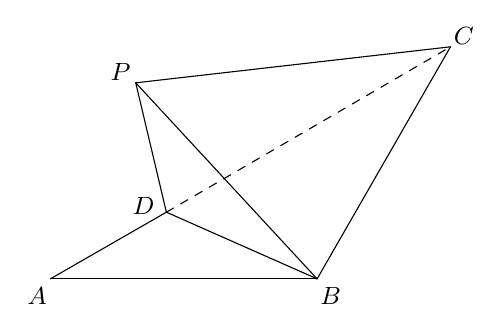
\begin{tikzpicture}[line cap=round,line join=round,font=\small,x=0.03515cm,y=0.03515cm]
% ===== 虚线先画（不可见棱 DC）=====
\draw[dash pattern=on 2.99pt off 2.99pt] (41.91,24.09)--(144.54,83.83);
% ===== 实线 =====
\draw (0,0)--(96.36,0);              % A-B
\draw (0,0)--(41.91,24.09);          % A-D
\draw (96.36,0)--(41.91,24.09);      % B-D
\draw (41.91,24.09)--(30.84,70.82);  % D-P
\draw (30.84,70.82)--(144.54,83.83); % P-C
\draw (30.84,70.82)--(96.36,0);      % P-B
\draw (96.36,0)--(144.54,83.83);     % B-C
% ===== 标注（照源字形框中心，显式坐标）=====
\node[anchor=center,inner sep=0] at (-4.73,-6.06) {\(A\)};
\node[anchor=center,inner sep=0] at (101.26,-6.06) {\(B\)};
\node[anchor=center,inner sep=0] at (149.35,87.67) {\(C\)};
\node[anchor=center,inner sep=0] at (33.70,26.40) {\(D\)};
\node[anchor=center,inner sep=0] at (25.38,74.66) {\(P\)};
\end{tikzpicture}
